\documentclass[14pt,a4paper]{report}

\usepackage{cmap}
\usepackage[warn]{mathtext}
\usepackage[utf8x]{inputenc}
\usepackage[T1,T2A]{fontenc}
\usepackage[english,russian]{babel}
\usepackage{indentfirst}
\usepackage{amsmath}
\usepackage{amsfonts}
\usepackage{amssymb}
\usepackage{graphicx}
\graphicspath{{image/}}
\usepackage{listings}
\usepackage{hyperref}
\usepackage{float}
\usepackage{fontspec}
\usepackage{placeins}
\setmainfont{SFNS Display}
\setmonofont{SFNS Display}

\lstset{
	inputencoding=utf8x,
	extendedchars=\true,
	frame=single,
	breaklines=true,
	numbers=left,
	keepspaces = true}

\voffset -24.5mm
\hoffset -5mm
\textwidth 173mm
\textheight 240mm
\oddsidemargin=0mm \evensidemargin=0mm


\begin{document}
	\begin{titlepage}
\begin{center}

\textbf{Санкт-Петербургский политехнический университет Петра Великого}

\vspace{5mm}
Институт компьютерных наук и технологий

\vspace{5mm}
Кафедра компьютерных систем и программных технологий

\vspace*{\fill}

\huge{Курсовой проект}

%\Large{о лабораторной работе №1}

\large{по дисциплине: <<Проектирование операционных систем>>}

\vspace*{2mm}
\large{Тема: <<Разработка демона звонков>>}

\vspace*{\fill}
\end{center}

%\begin{flushright}
\begin{large}
\hspace{0.4\linewidth} \textbf{Работу выполнил студент}

\vspace{5mm}
\hspace{0.4\linewidth} 13541/4 \hspace{1cm} \textit{Зорин А. Г.}

\vspace{3mm}
\hspace{0.4\linewidth} \textbf{Преподаватель}

\vspace{5mm}
\hspace{0.4\linewidth} \underline{\hspace{2cm} } \hspace{3mm} \textit{Душутина Е.В.}
\end{large}
%\end{flushright}

\vspace*{3cm}

\begin{center}
\normalsize Санкт-Петербург\\2017
\end{center}
\end{titlepage}

	\renewcommand{\thesection}{\arabic{section}}
	\setcounter{page}{2}
	\tableofcontents
	\pagebreak
	
	\setcounter{totalnumber}{10}
	\setcounter{topnumber}{10}
	\setcounter{bottomnumber}{10}
	\renewcommand{\topfraction}{1}
	\renewcommand{\textfraction}{0}
	
	\section{Цель работы}
Целью данной работы является разработка мобильного оконного менеджера. Оконный менеджер должен иметь строку состояния и рабочий стол, с которого можно запускать остальные приложения.
	\section{Описание задачи}
Данная курсовая работа выполнена в раках проекта по разработке мобильного устройства  на платформе Raspberry Pi Zero~\cite{RPiZero}. Данный проект включает в себя несколько задач:
\begin{itemize}
\item разработка аппаратной платформы мобильного устройства на основе Raspberry Pi Zero --- подбор необходимых компонентов мобильного устройства (GSM модуль, динамик, микрофон, аккумулятор и т.д.) и их размещение на плате устройства
\item установка и конфигурирование ОС для Raspberry Pi
\item разработка стека драйверов для комплектующих
\item разработка сервисного слоя (в виде демонов UNIX), который будет предоставлять необходимую информацию клиентским приложениям
\item \textbf{разработка мобильного оконного менеджера}, который позволит запускать и отображать на экране графические пользовательские приложения
\item разработка клиентских приложений (для осуществления звонков, настроек и т.д.)
\end{itemize}

Архитектура разрабатываемого проекта приведена на рисунке~\ref{fig:architecture}.
\begin{figure}[h!]
\center{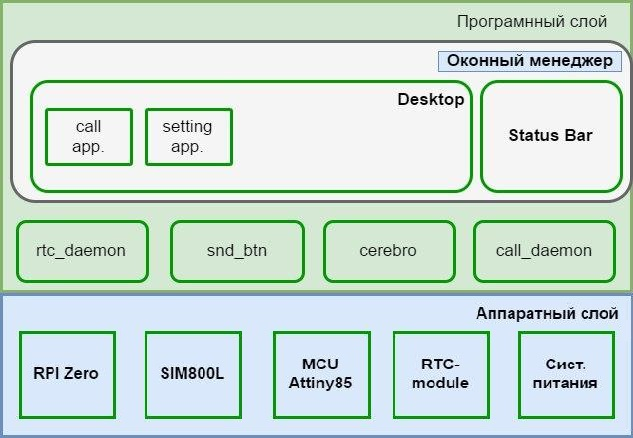
\includegraphics[width=\linewidth]{architecture}}
\caption{Архитектура проекта}
\label{fig:architecture}
\end{figure}

Таким образом, конечной целью разработки оконного менеджера~(ОМ) является его запуск на Raspberry Pi Zero. Необходимо учесть, что Raspberry обладает малой вычислительной мощностью, поэтому ОМ должен быть реализован как можно более оптимальным образом.

Мобильный ОМ должен так же иметь два встроенных системных приложения:
\begin{itemize}
\item строка состояния, которая отображает информацию об устройстве (текущее время, уровень заряда, уровень сигнала и т.д.). Строка состояния всегда отображается в верхней части экрана
\item рабочий стол, на котором расположены иконки запуска приложений, установленных в системе. Рабочий стол отображается на всю часть экрана, не занятую строкой состояния
\end{itemize}
Данные системные приложения не являются непосредственной частью ОМ. ОМ автоматически запускает их при своем запуске, и запоминает их идентификаторы для соответствующего отображения. ОМ должен иметь возможности указания путей к приложениям строки состояния и рабочего стола (т.е. должен иметь возможность конфигурирования).

При запуске несистемных приложений ОМ скрывает рабочий стол, выводит запущенное приложение на передний план и делает его активным. ОМ должен поддерживать три типа окон:
\begin{itemize}
\item обычные окна приложений, которые отображаются во весь экран
\item всплывающие уведомления (например, контекстное меню при нажатии правой кнопки мыши), которые отображаются в соответствии со своими размерами в указанной точке. Например, при нажатии на правую кнопку мыши открывается контекстное меню в точке нажатия с необходимыми размерами
\item окна меню (например стандартные меню типа "Файл" и т.д. в верхней части приложений). Должны запускаться в соответствии со своими размерами и отрисовываться начиная с нажатой кнопки.
\end{itemize}

Созданный оконный менеджер так же должен иметь возможность обработки управляющих комбинаций клавиш для:
\begin{itemize}
\item закрытия приложения
\item завершения работы ОМ
\item перелистывания окон
\item запуска терминала
\end{itemize}

Так же ОМ должен иметь возможности перемещения и изменения размеров окон.
	\section{Теоретические сведения}
\subsection{D-Bus}
D-Bus представляет из себя систему межпроцессорного взаимодействия, которая позволяет приложениям, находящимся в операционной системе (ОС), общаться между собой. D-Bus является частью проекта freedesktop.org~\cite{freedesktop}. Данная система обладает высокой скоростью работы, не зависит от рабочей среды и работает на POSIX-совместимых ОС.

D-Bus предоставляет несколько шин:
\begin{itemize}
\item Системная шина. Создается при старте демона D-Bus. С ее помощью происходит общение между различными демонами. 
\item Сессионная шина. Создается для пользователя, авторизовавшегося в системе. Для каждой сессионной шины запускается отдельная копия демона. Посредством этой копии общаются приложения, с которыми работает пользователь.
\end{itemize}

Каждое сообщение, передоваемое по шине, имеет своего отправителя. В том случае, когда сообщение не является широковещательным сигналом, оно имеет, в добавок к отправителю, своего получателя. Адреса отправителей и получаетлей, в контексте D-Bus, называются путями объектов по той причине, что каждое приложение состоит из набора объектов и сообщение происходит именно между этими объектами, а не между приложениями.

D-Bus также предусматривает концепцию сервисов. Сервис — уникальное местоположение приложения на шине. Приложение, при запуске, регистрирует один или несколько сервисов, которыми оно будет владеть до тех пор, пока самостоятельно не освободит. До этого момента никакое другое приложение, претендующее на тот же сервис, занять его не сможет. Именуются сервисы аналогично интерфейсам. После закрытия приложения ассоциированные сервисы также удаляются, а D-Bus посылает сигнал о том, что сервис закрыт.

Сервисы делают доступной ещё одну функцию — запуск необходимых приложений в случае поступления сообщений для них. Для этого должна быть включена автоактивация, а в конфигурации D-Bus за этим сервисом должно быть закреплено одно приложение.

После подключения к шине, приложение должно указать, какие сообщения оно желает получать, путём добавления масок совпадений (matchers). Маски представляют собой наборы правил для сообщений, которые будут доставляться приложению. Фильтрация может основываться на интерфейсах, путях объектов и методах.

Сообщения в D-Bus бывают четырёх видов: \textit{вызовы методов}, \textit{результаты вызовов методов}, \textit{сигналы (широковещательные сообщения)} и \textit{ошибки}.

В D-Bus у каждого объекта своё уникальное имя, которое выглядит как путь в файловой системе. Архитектура D-Bus показана с импользованием D-Bus интерфейса \textit{org.freedesktop.DBus.ObjectManager} на рис. \ref{fig:dbus}.
\begin{figure}[H]
\center{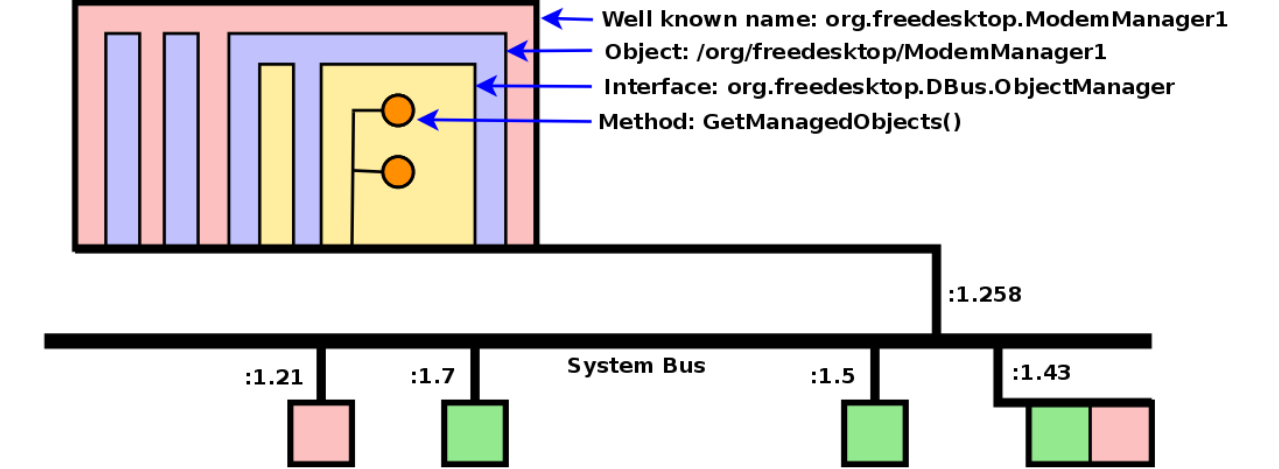
\includegraphics[width=0.6\linewidth]{dbus}}
\caption{Архитектура D-Bus}
\label{fig:dbus}
\end{figure}
\subsection{oFono}
Для организации общения с используемым sim-модулем был использолван программный проект oFono. Данный проект является бесплатным и распространяется под лицензией GNU GPL v2~\cite{oFono}. Проект oFono построен на стандарте 3GPP (3rg Generation Partnership Project) и использует D-Bus API для общения. Архитектура проекта oFono показана на рис. \ref{fig:ofono}.
\begin{figure}[H]
\center{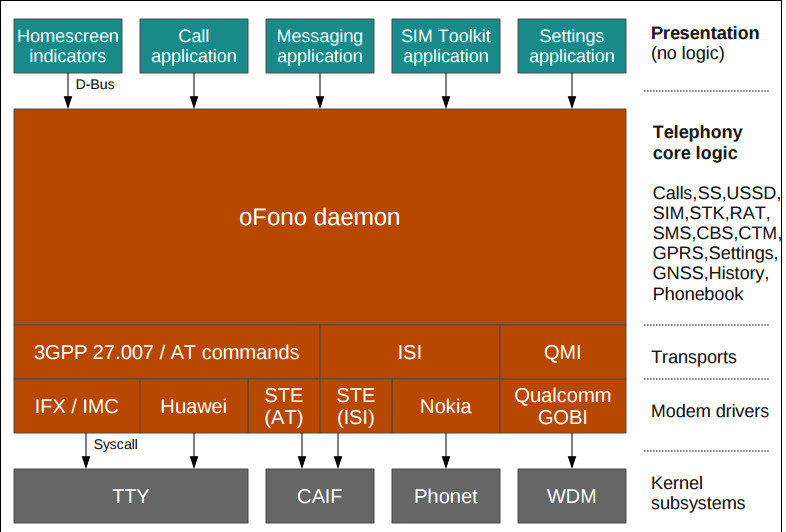
\includegraphics[width=0.6\linewidth]{ofono}}
\caption{Архитектура ofono}
\label{fig:ofono}
\end{figure}

Проект oFono был анонсирован компаниями Intel и Nokia в мая 2009 года. Последняя версия 1.4 была представлена в августе 2016 года. Работа над данным проектом ведется до сих пор. Исходные коды oFono находятся в свободном доступе, в гит репозитории.

Программный стек oFono поддерживает различные модули, такие как:
\begin{itemize}
\item 2G/3G
\item LTE
\item CDMA(Code-division multiple access)
\item GSM
\item Bluetooth и т.д.
\end{itemize}

Общаение между oFono и sim-модулем будет производится через различные AT-команды. В свою очередь, разрабатываемый демон будет общаться с oFono посредством D-Bus.

	\section{Анализ способов общения через D-Bus}
\subsection{QtDbus}
Qt --- это кросплатформенный инструментарий разработки программного обеспечения (ПО) на языке программирования \textit{C++}~\cite{Qt}. Qt позваляет запускать различные приложения, написанные с его помощью, на различных ОС, без необходимости переписывать исходный код. Одна из основных отличительных особенностей Qt - использование \textit{Meta Object Compiler (MOC)}. MOC - система предварительной обработки исходного кода. Она позволяет во много раз увеличить мощь библиотек вводя таки понятия, как \textit{слоты} и \textit{сигналы}. 

Qt позволяет создавать собственные плагины и размещать их непосредственно в панели визуального редактора. Также существует возможность расширения привычной функциональности виджетов, связанной с размещением их на экране, отображением, перерисовкой при изменении размеров окна.

Одним из весомых преимуществ проекта Qt является наличие качественной документации. Статьи документации снабжены большим количеством примеров. Исходный код самой библиотеки хорошо форматирован, подробно комментирован и легко читается, что также упрощает изучение Qt.

Помимо <<чистого>> Qt, для реализации графического интерфейса можно использовать связку \textit{Qt + QML}. QML представляет из себя декларативный язык программирования, основанный на \textit{JavaScript}, предназначенный для создания дизайна приложений. QML документ выглядит как дерево элеиентов. Сам QML элемент представляет из себя совокупность блоков:
\begin{itemize}
\item Графических
	\begin{itemize}
	\item Rectangle
	\item Image и т.д.
	\end{itemize}
\item Поведенческих
	\begin{itemize}
	\item State
	\item Transition
	\item Animation и т.д.
	\end{itemize}
\end{itemize}

Qt обеспечивает возможностью работать с D-Bus через собственный модуль, который называется QtDBus. Данный модуль полностью инкапсулирует низкоуровневую концепцию обмена сообщений в более простую - объектно ориентированную модель. Для работы с данном модулем существует огромное количество классов, каждый из которых хорошо задокументирован.

\subsection{GLib}
GLib --- набор из низкоуровневых системных библиотек, написанных на языке программирования \textit{C} и разрабатываемых, в основном, \textit{GNOME}~\cite{gnome}. Исходные коды GLib были отделены от GTK+ и могут быть использованы ПО отличным от \textit{GNOME}. GLib распространяется под лицензией GNU GPL и исходные коды находятся на \textit{github}.

GLib предоставляет такие структуры данных, как:
\begin{itemize}
\item Одно- и двусвязные списки
\item Хэш-таблицы
\item Динамические массивы
\item Динамическиие строки
\item Сбалансированные двоичные деревья и т.д.
\end{itemize}

Основные моменты D-Bus, в библиотеках GLib реализованы двумя, приблизительно идентичными, путями: \textit{dbus-glib} и \textit{GDBus}. В обеих реализациях прокси классы и вызовы методов D-Bus реализованы в виде объектов. Однако, существуют некоторые различия:
\begin{itemize}
\item \textit{dbus-glib} использует реализацию \textit{libdbus}. \textit{GDBus}, в отличии от \textit{dbus-glib} использует \textit{GIO} потоки в качестве транспортного уровня и имеет собственную реализацию для настройки подключения и аутентификации D-Bus. Помимо использования потоков в качестве транспорта, \textit{GDBus} позволяет избежать некоторых проблем связанных с многопоточными функциями.
\item \textit{dbus-glib} использует систему типа \textit{GObject} для аргументов методов, возвращаемых значений, а также - механизма сигналов. \textit{GDbus}, в свою очередь, пологается на систему типа \textit{GVariant}, которая разработана для соответствия типам D-Bus. 
\item \textit{dbus-glib} моделирует только интерфейсы D-Bus и не предоставляет никаких типов для объектов. \textit{GDBus} моделирует интерфейсы D-Bus (через типы \textit{GDBusInterface}, \textit{GDBusProxy} и \textit{GDBusInterfaceSkeleton}) и объекты (через типы \textit{GDBusObject}, \textit{GDBusObjectSkeleton} и \textit{GDBusObjectProxy}).
\item \textit{GDBus} предоставляет встроенную поддержку для org.freedesktop.DBus.Properties через тип \textit{GDBusProxy} и интерфейсы org.freedesktop.DBus.ObjectManager D-Bus, \textit{dbus-glib} - нет.
\item Типичный способ экспорта объекта с помощью \textit{dbus-glib} включает создание кода из данных XML с использованием \textit{dbus-binding-tool}. \textit{GDBus} предоставляет аналогичный инструмент под названием \textit{gdbus-codegen}, который также может генерировать Docbook D-Bus документацию интерфейсов.
\item \textit{dbus-glib} не предоставляет каких-либо удобных API для просмотра имен шин, \textit{GDBus} предоставляет семейство удобных функций \textit{g\_bus\_own\_name} и \textit{g\_bus\_watch\_name}.
\item \textit{GDBus} предоставляет API для анализа, генерации и работы с XML, \textit{dbus-glib} - нет.~\cite{freedesktop}
\end{itemize}

\subsection{Сравнение QtDBus и GLib}
В предыдущих секциях были рассмотренны такие спосбоы общения по D-Bus, как \textit{QtDBus}, \textit{GDBus}, \textit{dbus-glib}. Если проводить аналогию между рассмотренными библиотеками, то можно сделать вывод о том, что \textit{QtDBus} и \textit{GDBus} очень похожи между собой, а различия между \textit{GDBus} и \textit{dbus-glib} были рассмотренны в секции выше. Таким образом, в качестве общего заключения можно сделать вывод о том, что \textit{dbus-glib} является более низкоуровневой библиотекой для общения с D-Bus, чем \textit{QtDBus} или \textit{GDBus}.

	\section{Выполнение работы}
\subsection{Описание тестового стенда}
Для выполнения работы использовалось два тестовых стенда:
\begin{itemize}
\item Платформа Raspberry Pi 1 с ОС ArchLinux
\item Виртуальная машина с Arch Linux
\end{itemize}

Благодаря тому, что платформы Raspberry Pi 1 и Raspberry Pi Zero аппаратно полностью совместимы, ОМ разработанный на платформе RPi 1 будет совместим с RPi Zero. Однако, проблема в том, что RPi имеет проприетарную графику, которая не поддерживается в Wayland. Поэтому, задача конфигурирования ОС на платформе RPi включала в себя установку драйвера VC4~\cite{vc4}, который позволяет представить видеокарту RPi как стандартное DRI устройство.

Виртуальная машина c ArchLinux была установлена в гипервизоре VirtualBox. Однако, из-за того что в VirtualBox не реализована поддержка протокла Wayland, мобильный оконный менеджер запускался в качестве X-клиента в оконном менеджере xfce4.

\subsection{Выбор библиотеки-композитора}
Как было сказано ранее, в архитектуре Wayland оконный менеджер обязательно должен включать в себя композитор (в отличие от X). Так как реализация собственного Wayland-композитора с нуля --- задача слишком объемная и трудоемкая, был решено использовать какую-либо библиотеку-композитор. В таком случае задачей разработанного ОМ будет управление окнами.

Из проанализированных библиотек было решено выбрать библиотеку wlc по нескольким причинам:
\begin{itemize}
\item API библиотеки устойчив и проверен
\item на ее основе уже реализовано некоторое количество программ
\item для библиотеки есть некоторое количество примеров
\end{itemize}

\subsection{Разработка оконного менеджера}
Исходный код основного файла оконного менеджера приведен в листинге~\ref{lst:main}. В основной функции приложения main производятся следующие действия:
\begin{itemize}
\item анализируются аргументы командной строки (строки 358-365)
\item считывается конфигурация (строка 367)
\item устанавливаются функции-обработчики действий для wlc (строки 370-392)
\item инициализируется композитор (строки 395-397)
\item запускаются системные приложения (строка состояния и рабочий стол) (строки 399-425)
\item запускается оконный менеджер (строка 426)
\end{itemize}

Созданное приложение принимает один аргумент --- файл конфигурации. Если аргумент не указан, ищется и открывается файл по-умолчанию -- \texttt{~/.config/xxwm}. Пример конфигурационного файла приведен в листинге \ref{lst:conf}. В нем указываются пути к исполняемым файлам строки состояния и рабочего стола.

\begin{lstlisting}[label=lst:conf, caption={Формат конфигурационного файла ОМ}]
[statusbar]
exe=/home/kivi/workspace/Phone/src/status_bar/status

[desktop]
exe=/home/kivi/workspace/Phone/src/desktop/desktop
\end{lstlisting}

Считывание конфигурационного файла производится с помощью библиотеки inih. Исходные коды функций, которые производят считывание конфигурационного файла приведены в листингах \ref{lst:confh} -- \ref{lst:confc}.

Далее в функции main устанавливаются функции-обработчики для библиотеки-композитора. Данные функции обрабатывают события, получаемые от композитора и, соответственно, работают с типами данных композитора.  Композитор определяет несколько абстракций:
\begin{itemize}
\item output --- вся область отображения на экран. В терминах оконных менеджеров это соответствует "рабочему столу"
\item view --- окно приложения
\end{itemize}

Рассмотрим все эти функции более подробно.
\begin{itemize}
\item \texttt{wlc\_log\_set\_handler} устанавливает функцию, которая будет осуществлять логирование. В нашем случае устанавливается функция, которая просто выводит все сообщения в терминал с использованием функции \texttt{printf} (строчки 352-355).

\item \texttt{wlc\_set\_output\_resolution\_cb} устанавливает функцию, которая обрабатывает изменение разрешения экрана. Устанавливаемая функция \texttt{output\_resolution} просто вызывает функцию перерисовки окон \texttt{relayout} (строчки 174-177).

\item \texttt{wlc\_set\_view\_created\_cb} устанавливает функцию, которая будет вызываться при создании нового окна. Устанавливаемая функция \texttt{view\_created} устанавливает окну необходимые флаги, выносит окно на первый план, переключает фокус на это окно и вызывает функцию перерисовки (строки 180-192).

\item \texttt{wlc\_set\_view\_destroyed\_cb} устанавливает функцию, которая будет вызваться при уничтожении окна. Устанавливаемая функция \texttt{view\_destroyed} устанавливает фокус на самое верхнее окно и вызывает функцию перерисовки (строки 195-200).

\item \texttt{wlc\_set\_view\_focus\_cb} устанавливает функцию, которая отвечает за установку фокуса на окно. Устанавливаемая функция \texttt{view\_focus} устанавливает окну флаг \texttt{WLC\_BIT\_ACTIATED} (строчки 203-206).

\item \texttt{wlc\_set\_view\_request\_move\_cb} устанавливает функцию, которая отвечает за перемещение какого-либо окна по экрану. Устанавливаемая функция \texttt{view\_request\_move} вызывает функцию \texttt{start\_interactive\_move} (строчка 210), которая в свою очередь начинает интерактивное действие вызвав функцию \texttt{start\_interactive\_action} (строчка 42).  Функция \texttt{start\_interactive\_action} сохраняет параметры окна, на котором начато интерактивное действие, в глобальную переменную и выводит это окно на первый план (строчки 26-38).

\item \texttt{wlc\_set\_view\_request\_resize\_cb} устанавливает функцию, которая отвечает за изменение размеров окна. Устанавливаемая функция \texttt{view\_request\_resize} начинает интерактивное действие изменения окна вызывая функцию \texttt{start\_interactive\_resize} (строчка 215). Данная функция начинает интерактивное действие вызвав функцию \texttt{start\_interactive\_action}, а затем определяет то, какую грань окна необходимо перемещать (строчки 46-66). Так же данная функция устанавливает окну флаг \texttt{WLC\_BIT\_RESIZING}, который указывает на то, что окно в текущий момент меняет свой размер.

\item \texttt{wlc\_set\_view\_request\_geometry\_cb} устанавливает функцию, которая отвечает за установку указанному окну определенных размеров. Устанавливаемая функция \texttt{view\_request\_geometry} не делает ничего, так как ОМ не предполагает возможности изменять размер окна извне.

\item \texttt{wlc\_set\_keyboard\_key\_cb} устанавливает функцию-обработчик нажатий клавиатуры. Устанавливаемая функция \texttt{keyboard\_key} считывает код нажатой клавиши, флаги модификаторов (CTRL, ALT и т.д.) и обрабатывает следующие комбинации (строчки 225-266):
\begin{itemize}
\item CTRL+q --- закрытие активного окна (если это не системное приложение)
\item CTRL+стрелка вниз --- переключиться на следующее окно (аналог ALT+Tab в Windows)
\item CTRL+Escape --- завершить работу оконного менеджера
\item CTRL+Enter --- запустить терминал
\end{itemize}

\item \texttt{wlc\_set\_pointer\_button\_cb} устанавливает функцию-обработчик нажатий кнопок мыши. Устанавливаемая функция \texttt{pointer\_button} обрабатывает следующие комбинации (строчки 268-291):
\begin{itemize}
\item CTRL+ЛКМ --- переместить окно
\item CTRL+ПКМ --- изменить размеры окна
\end{itemize}

\item \texttt{wlc\_set\_pointer\_motion\_cb} устанавливает функцию-обработчик передвижения мыши. Устанавливаемая функция \texttt{pointer\_motion} проверяет, если в данный момент выполняется интерактивное действие, она соответствующим образом изменяет отображение активного окна (передвигает или изменяет размеры, в зависимости от выполняемого действия) (строчки 294-350).
\end{itemize}

Далее в функции main выполняется запуск системных приложений (строки состояния и рабочего стола) и запуск самого композитора. При этом, ОМ запоминает PID системных приложений для возможности их идентификации. Например, на основе этих PID ОМ решает можно ли закрывать соответствующее окно.

Одной из самых главных функций ОМ является функция перерисовки окно \texttt{relayout} (строки 90-171). Данная функция действует по следующему алгоритму:
\begin{enumerate}
\item берет самое верхнее (переднее) окно
\item проверяем, является ли окно окном строки состояния
\item если да, то запоминаем идентификатор окна
\item если нет, то рисуем данное окно на весь экран, кроме верхней строчки высотой в 30 пикселей
\item обновляем окно строки состояния перерисовывая ее в верхних 30 пикселях экрана 
\end{enumerate}

Данный алгоритм позволяет каждый раз перерисовывать максимум два окно: активное окно приложения и окно строки состояния. Строку состояние необходимо перерисовывать, потому что в какой-то момент времени могло изменится разрешение экрана. Данный алгоритм позволяет снизить вычислительную нагрузку ОМ на систему. 

Так же при перерисовке окна учитываются флаги типа окна. Библиотека WLC определяет пять флагов окна. Экспериментальным путем было выяснено, что при работе ОМ появляются и должны по-особому отображаться только два типа окон:
\begin{itemize}
\item \texttt{WLC\_BIT\_UNMANAGED} --- окна меню
\item \texttt{WLC\_BIT\_POPUP} --- уведомления и контекстные меню (вызываемые при нажатии ПКМ)
\end{itemize}

Данные типы окон отображаются по-особому. Окна меню отображаются в соответствии с изначально заданными им параметрами, ничего не изменяется. Окна контекстных меню смещаются относительно координат их окна-родителя и координат нажатия мыши. Остальные окна отображаются по-умолчанию на всю область экрана, незанятую строкой состояния.

Примеры работы оконного менеджера приведены на рисунках \ref{fig:wm1} -- \ref{fig:wm4}.
\begin{figure}[h!]
\center{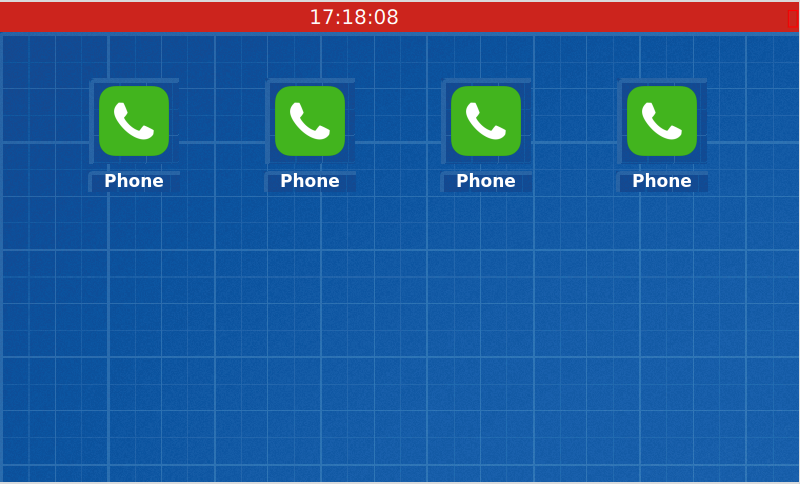
\includegraphics[width=\linewidth]{wm1}}
\caption{Оконный менеджер}
\label{fig:wm1}
\end{figure}
\begin{figure}[h!]
\center{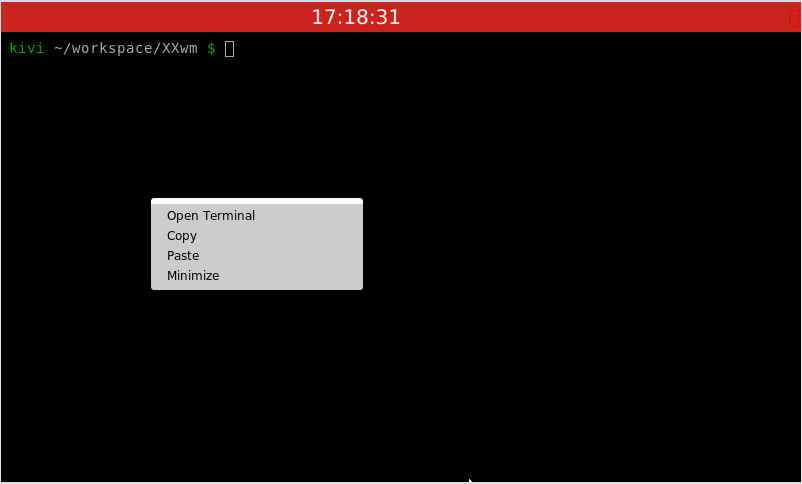
\includegraphics[width=\linewidth]{wm2}}
\caption{Отображение терминала и контекстного меню}
\label{fig:wm2}
\end{figure}
\begin{figure}[h!]
\center{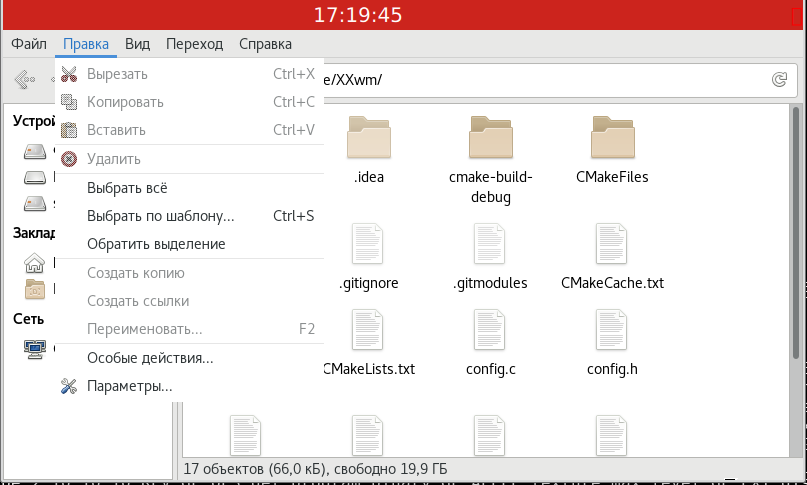
\includegraphics[width=\linewidth]{wm3}}
\caption{Отображение файлового менеджера и меню}
\label{fig:wm3}
\end{figure}
\begin{figure}[h!]
\center{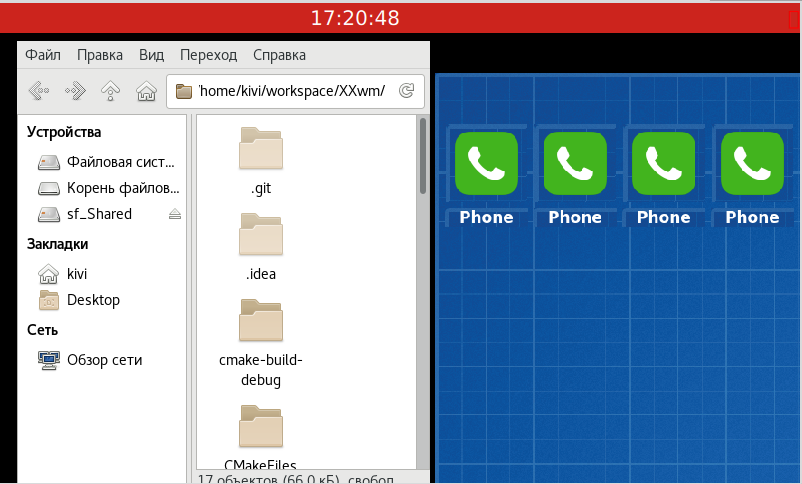
\includegraphics[width=\linewidth]{wm4}}
\caption{Перемещение и изменение размеров окон}
\label{fig:wm4}
\end{figure}

\subsection{Добавление ОМ в экранный менеджер}
Экранный менеджер или менеджер входа --- графический экран, который отображается в конце процесса загрузки вместо стандартного приглашения командной строки. Экранный менеджер представляет собой экран ввода имени пользователя и пароля для входа в систему. Существует большое количество экранных менеджеров, однако все они детектируют установленные в систему оконные менеджеры по конфигурационным файлам формата \texttt{.desktop}. Данные файлы являются неким подобием ярлыков в Windows. \texttt{.desktop} --- это сандартный для Linux конфигурационный файл. Подробное описание формата файлов \texttt{.desktop} приведено в~\cite{desktop}. Для созданного ОМ был создан минимальный файл \texttt{.desktop} (листинг \ref{lst:desktop}).
\begin{lstlisting}[label=lst:desktop, caption={Файл .desktop для ОМ}]
[Desktop Entry]
Name=XXwm
Comment=Mobile Wayland window manager
Exec=/home/kivi/workspace/XXwm/xxonwm
Type=Application
\end{lstlisting}

Для того, чтобы экранный менеджер смог обнаружить ОМ необходимо поместить \texttt{.desktop} в каталог \texttt{/usr/share/wayland-sessions/}. Для проверки данного файла был установлен экранный менеджер sddm. Пример выбора ОС в sddm приведен на рисунке \ref{fig:sddm}.
\begin{figure}[h!]
\center{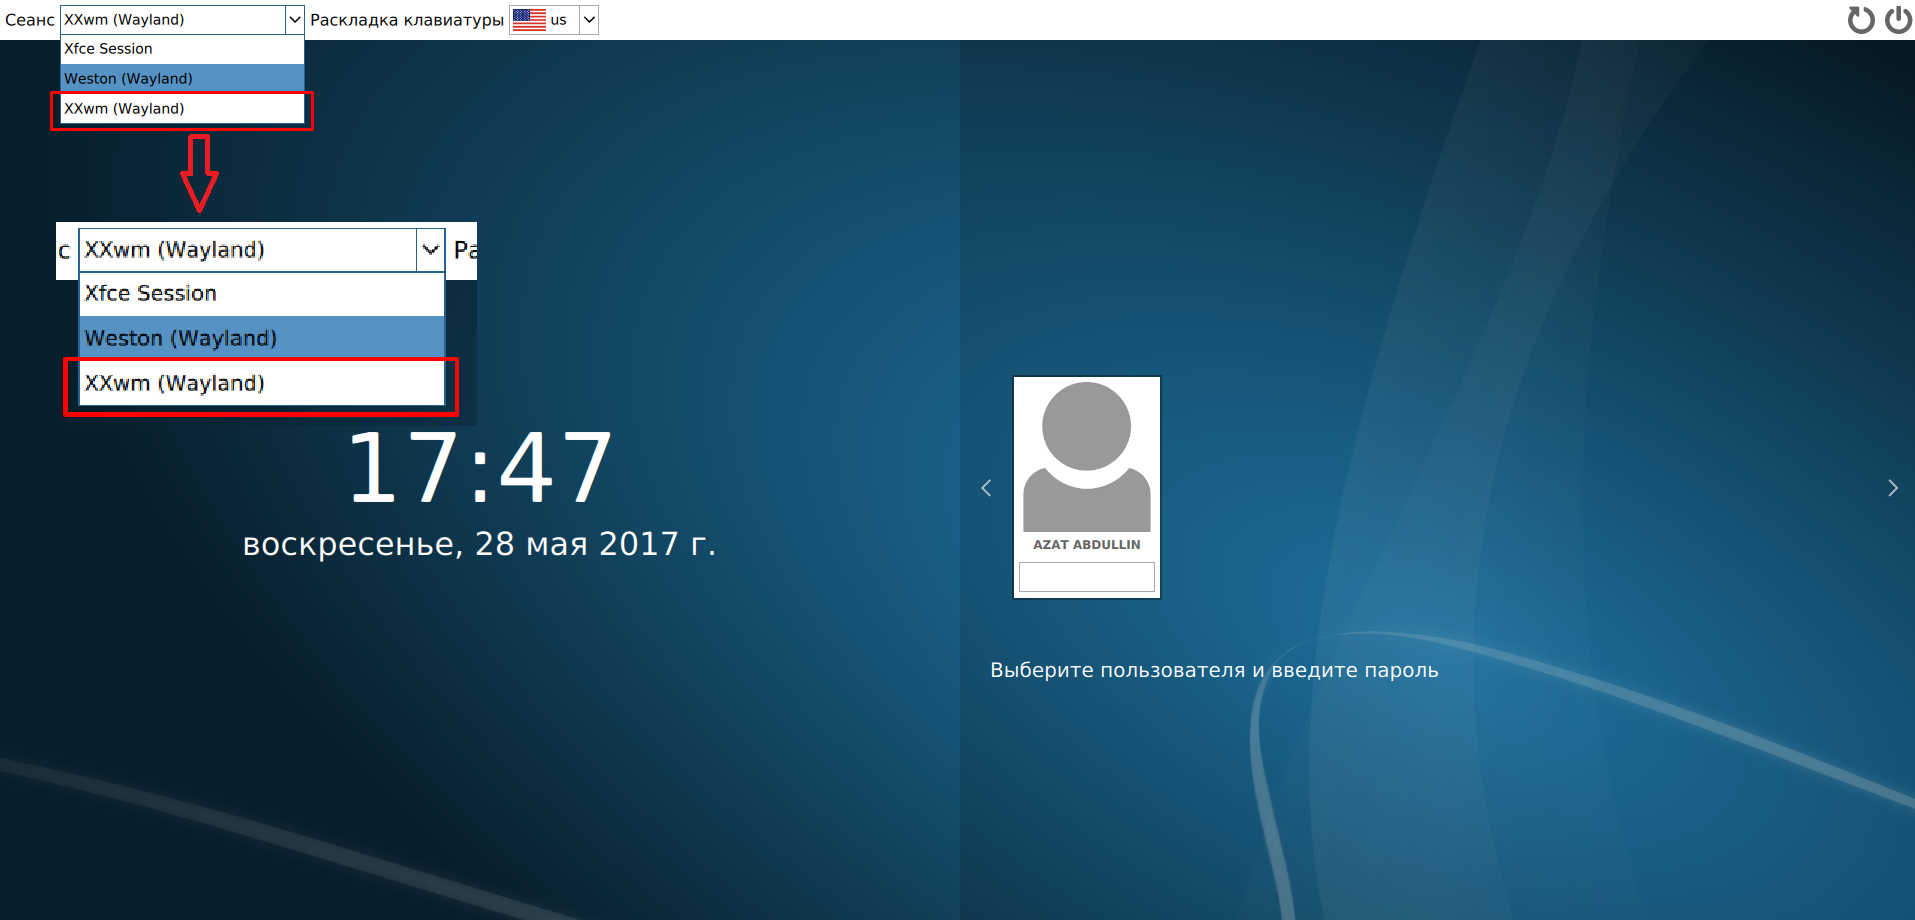
\includegraphics[width=\linewidth]{sddm}}
\caption{Пример загрузки ОМ через экранный менеджер}
\label{fig:sddm}
\end{figure}
	\section{Выводы}
В ходе работы были проанализированы и сравнены различные способы работы с D-Bus. В результате анализа, для организации работы была выбрана библиотека dbus-glib. Она позволяет облегчить работу платформы и увеличить производительность, так как явлеятся низкоуровневой и имеет низкий уровень абстракции. 
В данной работе был реализован демон звонков. Данный демон разрабатывался в рамках проекта по разработке смартфона. Разработанный демон позволяет отслеживать различные изменения голосовых вызовов, произошедших на используемом модуле SIM-808. Помимо демона звонков было разработано графическое приложение телефона. Созданный демон взаимодействует с данным приложением в зависимости от статуса звонка.

	\FloatBarrier
			
	\pagebreak
	\addcontentsline{toc}{section}{Список используемой литературы}
	\bibliography{biblio}
	\bibliographystyle{ugost2008}  %% стилевой файл для оформления по ГОСТу
	
	\pagebreak	
	\section{Прилагаемые материалы}
	Список прилагаемых материалов:
	\begin{itemize}
		\item Техническое задание.docx --- техническое задание на проект;
		\item progManual.pdf --- руководство системного программиста;
		\item sources.pdf --- текст программы;
		\item spec.pdf --- описание программы;
		\item tests.pdf --- программа и методика испытаний;
		\item userManual.pdf --- руководство пользователя.
	\end{itemize}
	
	
	\pagebreak
	\section*{Листинги}

\lstinputlisting[label=lst:main, caption={Файл main.cpp}, 
language={C}]{../src/daemon/main.cpp}

\lstinputlisting[label=lst:struct, caption={Файл Struct.h}, 
language={C}]{../src/daemon/Struct.h}

\lstinputlisting[label=lst:cmake, caption={Файл сборки CMakeLists.txt}, 
language={C}]{../src/daemon/CMakeLists.txt}

\lstinputlisting[label=lst:mainwindowgui, caption={Файл mainwindow.cpp}, 
language={C}]{../src/gui/mainwindow.cpp}

\lstinputlisting[label=lst:mainwindowh, caption={Файл mainwindow.h}, 
language={C}]{../src/gui/mainwindow.h}

\lstinputlisting[label=lst:mainqml, caption={Главное окно графического приложения}, 
language={C}]{../src/gui/qml/main.qml}

\lstinputlisting[label=lst:button, caption={Реализация класса Button}, 
language={C}]{../src/gui/qml/core/Button.qml}

\lstinputlisting[label=lst:phone, caption={Файл сборки phone.pro}, 
language={C}]{../src/gui/phone.pro}

\end{document}
